\documentclass{article}

\usepackage[english]{babel}
\usepackage{amsmath}
\usepackage{amssymb}
\usepackage{algorithm}
\usepackage{algpseudocode}
\usepackage{float}


% Set page size and margins
% Replace `letterpaper' with `a4paper' for UK/EU standard size
\usepackage[a4paper,top=2cm,bottom=2cm,left=3cm,right=3cm,marginparwidth=1.75cm]{geometry}

% Useful packages
\usepackage{amssymb}
\usepackage{siunitx}
\PassOptionsToPackage{hyphens}{url}\usepackage{hyperref}
\usepackage{cleveref}
\usepackage[utf8]{inputenc}
\usepackage{csquotes}
\usepackage{booktabs}
\usepackage{longtable}
\usepackage{adjustbox}
\usepackage{array}
\usepackage{url}
\usepackage{titlesec}
%\usepackage[compatibility=false]{caption}
\usepackage{authblk}
\usepackage{xcolor} % Load the xcolor package for color options
\renewcommand{\thetable}{\Roman{table}}

% Define a new format for \subsection
\titleformat{\subsection}
  {\mdseries\itshape\large} % Medium series, italic shape, and large font size
  {\thesubsection}{1em}{} % Numbering, spacing, and the section title itself


% Emerald Harvard Citation Style

\usepackage[english]{babel}
\usepackage[style=authoryear,backend=biber,natbib=true,maxcitenames=2,uniquelist=false]{biblatex}
\addbibresource{Bibliography.bib} % your .bib file

% Customizing biblatex for Harvard style
% Customizing biblatex for Harvard style
\DeclareNameAlias{sortname}{family-given}
\DeclareNameAlias{default}{family-given}

\renewbibmacro{in:}{}
\DeclareFieldFormat[article]{title}{\mkbibquote{#1}\addcomma}
\DeclareFieldFormat[book]{title}{\mkbibemph{#1}\addcomma}
\DeclareFieldFormat[bookinbook]{title}{\mkbibemph{#1}\addcomma}
\DeclareFieldFormat[inbook]{title}{\mkbibquote{#1}\addcomma}
\DeclareFieldFormat[incollection]{title}{\mkbibquote{#1}\addcomma}
\DeclareFieldFormat[inproceedings]{title}{\mkbibquote{#1}\addcomma}
\DeclareFieldFormat[manual]{title}{\mkbibemph{#1}\addcomma}
\DeclareFieldFormat[misc]{title}{\mkbibemph{#1}\addcomma}
\DeclareFieldFormat[thesis]{title}{\mkbibemph{#1}\addcomma}
\DeclareFieldFormat[unpublished]{title}{\mkbibquote{#1}\addcomma}
\DeclareFieldFormat[patent]{title}{\mkbibemph{#1}\addcomma}
\DeclareFieldFormat[report]{title}{\mkbibemph{#1}\addcomma}
\DeclareFieldFormat[online]{title}{\mkbibquote{#1}\addcomma}
\DeclareFieldFormat[software]{title}{\mkbibemph{#1}\addcomma}
\DeclareFieldFormat[booklet]{title}{\mkbibemph{#1}\addcomma}
\DeclareFieldFormat[periodical]{title}{\mkbibemph{#1}\addcomma}
\DeclareFieldFormat[standard]{title}{\mkbibemph{#1}\addcomma}

\DeclareFieldFormat[article]{journaltitle}{\iffieldundef{shortjournal}{\mkbibemph{#1}\addcomma}{\mkbibemph{\printfield{shortjournal}}\addcomma}}
\DeclareFieldFormat{volume}{\bibstring{volume}~#1}
\DeclareFieldFormat{number}{\bibstring{number}~#1}

% Definitions for "Vol." and "No."
\DefineBibliographyStrings{english}{
  volume = {Vol.},
  number = {No.}
}

\renewbibmacro*{volume+number+eid}{%
  \printfield{volume}%
  \setunit*{\addspace}%
  \printfield{number}%
  \setunit{\addcomma\space}%
  \printfield{eid}}

\renewbibmacro*{journal+issuetitle}{%
  \usebibmacro{journal}%
  \setunit*{\addcomma\space}%
  \usebibmacro{volume+number+eid}%
  \setunit{\addcomma\space}%
  \usebibmacro{issue+date}}

\renewbibmacro*{publisher+location+date}{%
  \printlist{publisher}%
  \iflistundef{location}
    {\setunit*{\addcomma\space}}
    {\setunit*{\addcolon\space}}%
  \printlist{location}%
  \setunit*{\addcomma\space}%
  \usebibmacro{date}}

\renewcommand*{\bibpagespunct}{\addcomma\space}

% Customizing page field format to prevent duplication
% \DeclareFieldFormat{pages}{%
%   \mkfirstpage[{\mkpageprefix[page]{#1}}]{#1}}

% Customizing citations for Harvard style
\DeclareCiteCommand{\cite}[\mkbibparens]
  {\usebibmacro{prenote}}
  {\usebibmacro{citeindex}%
   \usebibmacro{cite}}
  {\multicitedelim}
  {\usebibmacro{postnote}}

\renewbibmacro*{cite:labelyear+extrayear}{%
  \iffieldundef{labelyear}
    {}
    {\printtext[bibhyperref]{%
       \printfield{labelyear}%
       \printfield{extrayear}}}}

\renewbibmacro*{cite:labeldate+extradate}{%
  \iffieldundef{labelyear}
    {}
    {\printtext[bibhyperref]{%
       \printfield{labelyear}%
       \printfield{extradate}}}}

\AtEveryBibitem{
  \clearfield{month}
  \clearfield{day}
  \ifentrytype{book}{
    \clearlist{location}
  }{}
}

% Formatting "et al." in italics followed by a comma
\DefineBibliographyStrings{english}{
  andothers = {\textit{et al.},}
}

\DeclareFieldFormat[article]{volume}{\bibstring{jourvol}\addnbspace #1}
\DeclareFieldFormat[article]{number}{\bibstring{number}\addnbspace #1}
\DeclareFieldFormat[article]{volume}{Vol. #1}
\DeclareFieldFormat[article]{number}{No. #1}
% Customizing DOI field format to lowercase "doi"
%\DeclareFieldFormat{doi}{\bibstring{doi}\addcolon\space\url{#1}}

% Customizing URL field format to "available at:"
\DeclareFieldFormat{url}{\bibstring{available at}\addcolon\space\url{#1}}
\DeclareFieldFormat{urldate}{\mkbibparens{accessed \addspace#1}}

% Customizing urldate to match the required format
\DeclareFieldFormat{urldate}{%
  \mkbibparens{accessed\space%
    \thefield{urlday}\addspace%
    \mkbibmonth{\thefield{urlmonth}}\addspace%
    \thefield{urlyear}}}


% Configure cleveref
\crefformat{figure}{#2Figure~#1#3}
\Crefformat{figure}{#2Figure~#1#3}
\crefformat{table}{#2Table~#1#3}
\Crefformat{table}{#2Table~#1#3}
\crefformat{section}{#2Section~#1#3}
\Crefformat{section}{#2Section~#1#3}

%Front Matter
\author[1]{Suhani Surana}




\title{Solving time dependent Maxwell's Equations and 1D and 2D FDTD Simulation and Analysis of Electromagnetic Wave Propagation in Nonlinear Photonic Crystals}


\begin{document}

\maketitle

\section{Introduction}
\label{sec:introduction}
\textbf{Title} MW/M31 Galaxy Major Merger Remnant: Stellar remnant and formation of elliptical galaxies
\newline \newline
\textbf{Specific Research Questions} - Kinematics of the Merged Bulges and Disks: evolution of the rotation curve (“ob- served” and mass-derived), dispersion profile, angular momentum. How well is the remnant described as a classical elliptical galaxy based on kinematics? Is there any rotation?
\newline \newline \textbf{Proposed Topic - Analysing the kinematics of the MW/M31 Galaxy Major Merger Remnant.}


The study of major galaxy mergers and their kinematic impact on the remnant structure is a very important part of the galaxy evolution studies.  By analyzing the kinematics of merger remnants, we can trace the evolutionary pathways that lead to different structural and dynamical outcomes. The formation of ellipticals due to Major Mergers is something which can be found by analyzing the kinematics of the remnant structure.
Some of the results by analysing the kinematics are as follows. Compared to the remnants of dissipationless disc galaxy mergers, the remnants created by the collision of gas-rich disc galaxies are rounder, smaller, and have bigger rotation speeds and higher centre velocity dispersions. 
Dissipational merger may also provide a natural
mechanism to produce kinematic subsystems in elliptical galaxies \cite{1991SciAm.265b..40B}
\newline \newline One important thing that we know how gas-rich mergers can trigger intense starbursts, followed by quenching due to AGN and supernova feedback. The figure shows the Milky Way–Andromeda merger, highlighting our understanding of how an intragroup medium (IGM) accelerates mergers by enhancing dynamical friction. This process influences the final remnant’s kinematics, likely resulting in an elliptical galaxy. \cite{2008MNRAS.386..461C}
\newline \newline Some of the open questions include how surface brightness profiles, metallicities and
abundance ratios, and kinematic subsystems of our merger remnants of very distant galaxies and how it can used to further enhance our explanation of galaxy evolution.{\cite{Cox_2006}}
\begin{figure}[H]
    \centering
    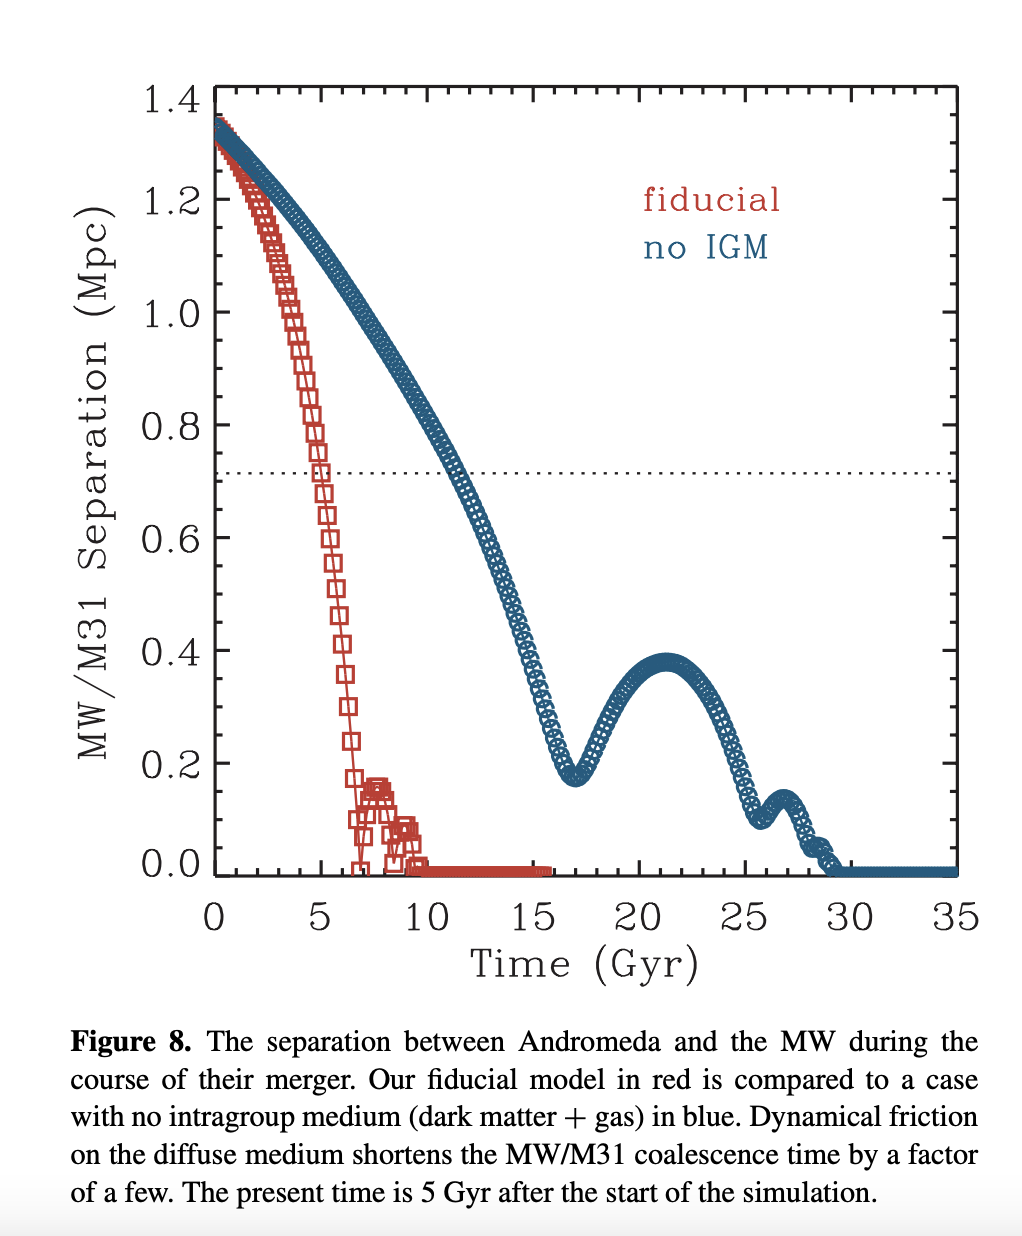
\includegraphics[width=0.5\linewidth]{Screenshot 2025-03-20 at 4.41.15 PM.png}
    \caption{The separation between the centres of Andromeda and the MW
during the course of their merger. }
    \label{fig:enter-label}
\end{figure}


\section{Method}
\label{sec:method}

\begin{itemize}
    \item To study the kinematics of the merger remnant, I will first identify simulation snapshots where the MW and M31 have fully merged and the system is dynamically relaxed.
    \item These snapshots will by the seperation plots in Homework 6. Using the formula (SN * 10)/0.7, I found out the snapshots numbers to be 280, 420 and 600. I will use high res as it would give me much better velocity dispersions as a function of r.
    
\end{itemize}
\begin{itemize}
    \item Extract stellar disk and bulge particles from both MW and M31.
    \item Concatenate them. 
\end{itemize} 

\begin{itemize}
    \item Compute the center of mass position  (\textbf{Reference: HW 2}) ($R_{\text{COM}}$) and velocity ($V_{\text{COM}}$) using:
    \begin{equation}
        \mathbf{R}_{\text{COM}} = \frac{\sum m_i \mathbf{r}_i}{\sum m_i}, \quad \mathbf{V}_{\text{COM}} = \frac{\sum m_i \mathbf{v}_i}{\sum m_i}
    \end{equation}
    \item Calculate positions and velocities to be in  the newly computed COM reference frame:
    \begin{equation}
        \mathbf{r}_i' = \mathbf{r}_i - \mathbf{R}_{\text{COM}}, \quad \mathbf{v}_i' = \mathbf{v}_i - \mathbf{V}_{\text{COM}}
    \end{equation}
    \item Then I would orient the galaxy edge on by orienting the angular momentum along the z axis and  create a phase diagram ($V_{\theta}$ vs. radius), with color coding to understand the direction of rotation and if at all rotation is happening. (Important thing is to extend the area to around 10-15 kpc to observe any true rotational effects)(\textbf{Reference: Lab 7})
    
    \item Also, will calculate  the observed and mass-derived rotation curves:
    \begin{equation}
        V_{c}(r) = \sqrt{\frac{G M(r)}{r}}
    \end{equation}
\end{itemize}

\begin{itemize}
    \item Calculate the velocity dispersion profile using half mass radius.
    
    \item Calculate the ratio of ordered to random motion ($V/\sigma$):
    \item If $V/\sigma \gg 1$, the system is a disk-like fast rotator.
    \item If $V/\sigma \ll 1$, it is a pressure-supported elliptical galaxy.
    
    \item Also, I will the total angular momentum of the remnant:
    \begin{equation}
        \mathbf{L} = \sum m_i (\mathbf{r}_i \times \mathbf{v}_i)
    \end{equation}
\end{itemize}

\begin{itemize}
    \item Apply the virial theorem to estimate total mass and compare it to the simulation data (\textbf{Reference: Lab 5}):
   
    \item Also I will check if the remnant follows the fundamental plane relation for elliptical galaxies and analyse it:
    \begin{equation}
        R_e \propto \sigma^2 \langle I \rangle^{-0.82}
    \end{equation}

\end{itemize}

\section{Hypothesis}

\begin{itemize}
    \item The MW/M31 merger remnant might exhibit  rotational support.  High velocity dispersion is expected due to the violent relaxation process which would be similar to  elliptical galaxies.  
    The MW/M31 merger remnant is expected to retain some rotation, but it will likely be a slow rotator due to the low gas content of both galaxies. The remnant may form a large bulge, and stellar populations might add complexity to the rotation profile. The dark matter halos will also influence the system's dynamics, potentially dampening rotation further, leading to a slower overall spin.
\end{itemize}


%\break
\printbibliography

\end{document}
